%%
%% Beuth Hochschule für Technik --  
%%
%% Kapitel 4 - 
%%
%%	

\newpage
[Perkowski]
\section{Messtechnische Identifikation des Störverhaltens der Strecke}\label{Kapitel4}
Da das Verhalten der Störübertragungsfunktion zu ermitteln ist, kann wie im Kapitel \ref{Kapitel3} vorgegangen werden. Die Strecke wird erst in den Arbeitspunkt erregt und dann die Störgröße mit einem Schalter an der Hardware zugeschaltet. Wir haben die Störmessung in der Datei \textit{stoer\_err.mat} aufgezeichnet.

\begin{figure}[h]
	\begin{center}
		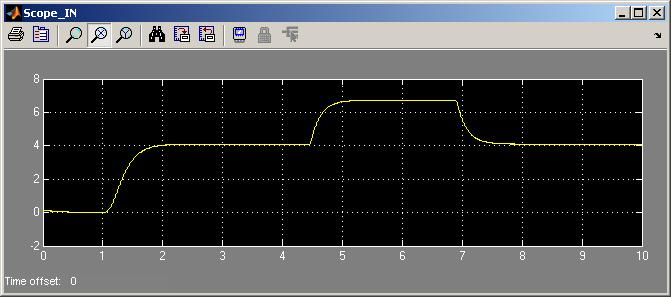
\includegraphics[scale=0.5]{stoerung.jpg}
		\caption{Strecke mit Störung}
       \label{stoer}
	\end{center} 
\end{figure}

Nachdem wir die gemessene Sprungantwort betrachtet haben, schlussfolgerten wir, dass es sich um PT1-System handeln muss. 
Da mit Hilfe des Tools \textit{sys\_id} die Zeitachsen einer Funktion eingegrenzt werden können, haben wir die Störung in zwei Glieder geteilt (einklingende Störung und abklingende Störung). Nach der Identifikation der beiden Teile der Störung, haben wir erkannt, dass sich die Teile annähernd gleichen. Die Ergebnisse können in den folgenden Abbildungen \ref{stoerfkt1} und \ref{stoerfkt2} nachvollzogen werden.

\newpage

Die ermittelte Störungsfunktion:

\begin{center}
$ G(s)_{stoer} = \dfrac{2,6424}{1 + 0,16207} $
\end{center}

\begin{figure}[h]
	\begin{center}
		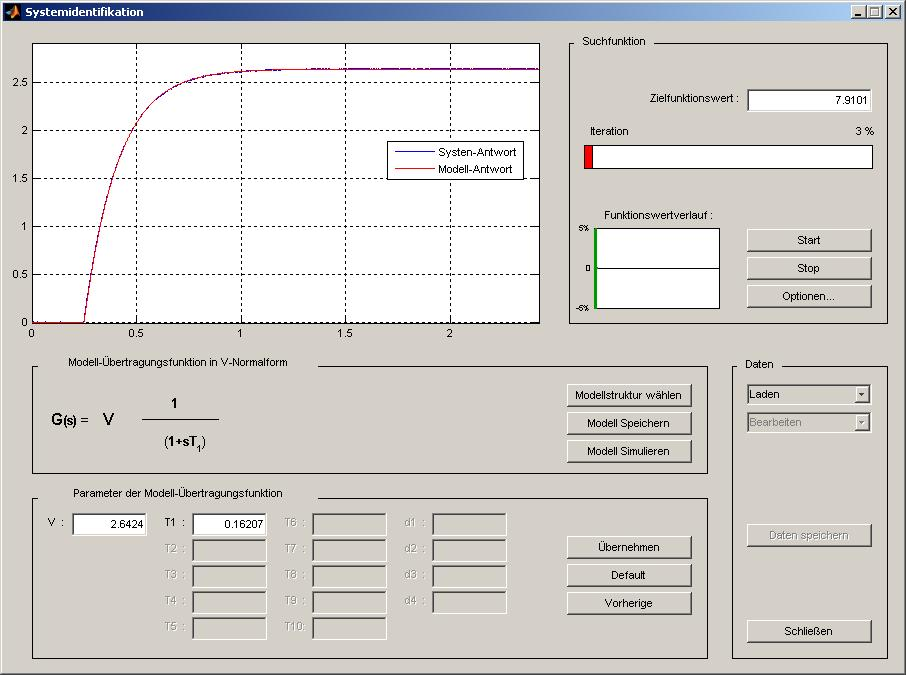
\includegraphics[scale=0.4]{stoerung_1_uebfkt.jpg}
		\caption{erster Ausschnitt Übertraungsfunktion mit Störung}
       \label{stoerfkt1}
	\end{center} 
\end{figure}

\begin{center}
$ G(s)_{stoer} = \dfrac{2,6433}{1 + 0,16367} $
\end{center}

\begin{figure}[h]
	\begin{center}
		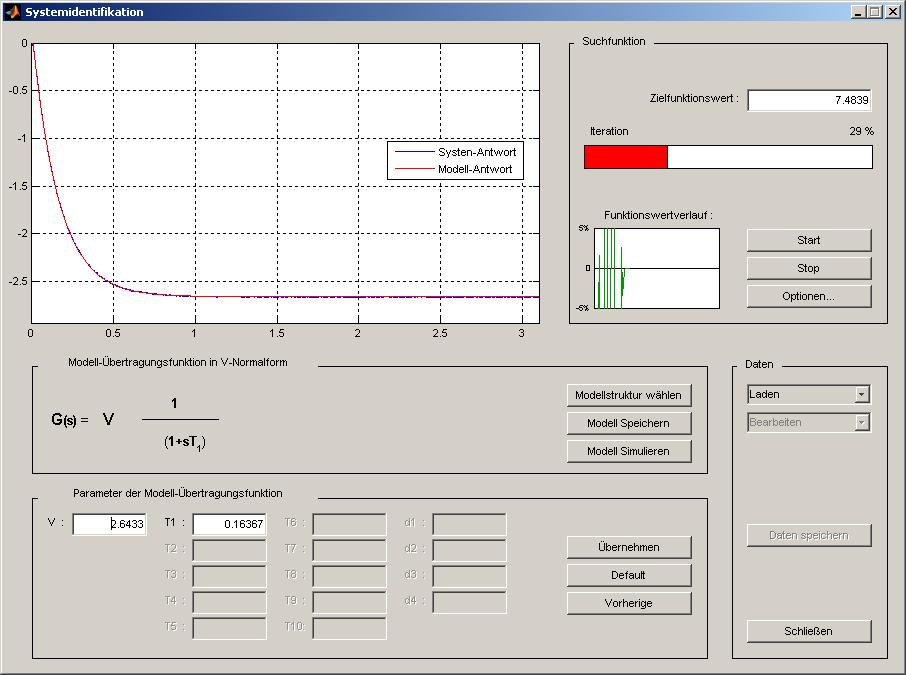
\includegraphics[scale=0.4]{stoerung_2_uebfkt.jpg}
		\caption{zweiter Ausschnitt Übertraungsfunktion mit Störung}
       \label{stoerfkt2}
	\end{center} 
\end{figure}

